
\documentclass[a4paper,12pt]{article}
\usepackage{graphicx}
%To use this font, you need XeTex or LuaTex, prefer openleaf
\newenvironment{codefont}{\fontfamily{ccr}\selectfont}{\par}

\title{
	\normalfont \normalsize 
	\textsc{Pimpri Chinchwad College of Engineering \\ 
		Computer Laboratory - IV} \\
	[10pt] 
	\rule{\linewidth}{0.5pt} \\[6pt] 
	\huge Assignment No - A3 \\
	\rule{\linewidth}{2pt}  \\[10pt]
}
\author{}
\date{\normalsize}


\begin{document}
\maketitle

%%%%%%%%%%%%%%%%%%%%%%%
% FOR A NUMBERED LIST
% \begin{enumerate}
% \item Your_Item
% \end{enumerate}
%%%%%%%%%%%%%%%%%%%%%%%
% FOR A BULLETED LIST
% \begin{itemize}
% \item Your_Item
% \end{itemize}
%%%%%%%%%%%%%%%%%%%%%%%
% TO IMPORT AN IMAGE
% \includegraphics[width=\textwidth]{name_of_file}
% \textwidth makes the picture the width of the paragraphs
%%%%%%%%%%%%%%%%%%%%%%%%%%%%%%
% TO CREATE A FIGURE WITH A NUMBER AND CAPTION
% \begin{figure}
% \includegraphics[width=\textwidth]{image}
% \caption{Your Caption Goes Here}
% \label{your_label}
% \end{figure}
% REFER TO YOUR FIGURE LATER WITH
% \ref{your_label}
% LABELS NEED TO BE ONE WORD
%%%%%%%%%%%%%%%%%%%%%%%%%%%%%
% TO ADD CODE
% \begin{codefont}
% Some code in "courier" font
%\end{codefont}
%%%%%%%%%%%%%%%%%%%%%%%%%%%%%
\section{Aim}
	\paragraph{} Write a MPI program for calculating a quantity called coverage from data files.
	
\section{Objective}
	\begin{itemize}
		\item To understand concept of Message Passing Interface(MPI) 
		\item	To effectively use multi-core or distributed, concurrent/Parallel environments.  
		\item	To develop problem solving abilities using Mathematical Modeling 
		
	\end{itemize}
	
\section{Mathematical Model}
	
	Let ,  
	S = \{ s, e, x, y, Fm, Si, DD, NDD \} \\
	s = Initial State, i.e. MPI\_Init() \\
	e = End State , i.e.MPI\_Finalize() \\
	Si = Intermediate states x = Input values i.e. Numbers in random manner\\
	 y = Output/Result. i.e. Sum of numbers  \\
	  Fm=Main function or algorithm that gives specific output \\
	   i.e. MPI\_Scatter(), MPI\_Gather(). 
	 NDD = Non deterministic data \\
	 DD = Deterministic data 
	
\section{Theory}
	\subsection{Concept of MPI}
		\paragraph{} MPI is a specification for the developers and users of message passing libraries. By itself, it is NOT a library - but rather the specification of what such a library should be. 
		
		MPI primarily addresses the message-passing parallel programming model: data is moved from the address space of one process to that of another process through cooperative operations on each process. 	 
		Simply stated, the goal of the Message Passing Interface is to provide a widely used standard for writing message passing programs. 
		
		The Message Passing Interface Standard (MPI) is a message passing library standard based on the consensus of the MPI Forum, which has over 40 participating organizations, including vendors, researchers, software library developers, and users. 	 
		The goal of the Message Passing Interface is to establish a portable, efficient, and flexible standard for message passing that will be widely used for writing message passing programs. MPI is not an IEEE or ISO standard, but has in fact, become the "industry standard" for writing message passing programs on HPC platforms. 
	
		
\subsection{MPI Programming Model:}	

		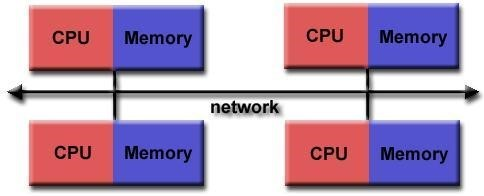
\includegraphics{MPI_01}

		  
		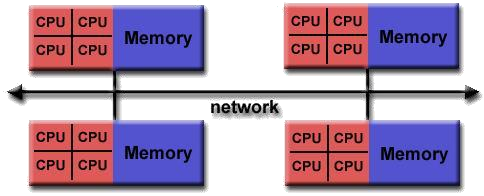
\includegraphics{MPI_02}
		\\
		\\
		Both the diagrams show the general programming model of the 
		MPI \\ system.
		
		

	\subsection{General MPI Programming Structure}
		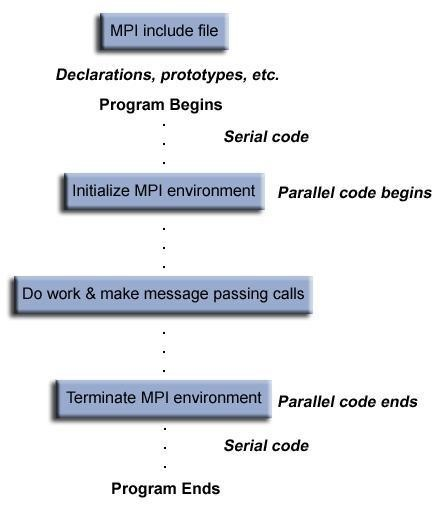
\includegraphics[width=\textwidth]{MPI_03}
\newpage		
\textbf{Communicators and Groups:} \\ \\
MPI uses objects called communicators and groups to define which collection of processes may communicate with each other.\\ \\
Most MPI routines require you to specify a communicator as an argument.\\ \\ 
MPI\_COMM\_WORLD whenever a communicator is required - it is the predefined communicator that includes all of your MPI processes. \\ \\

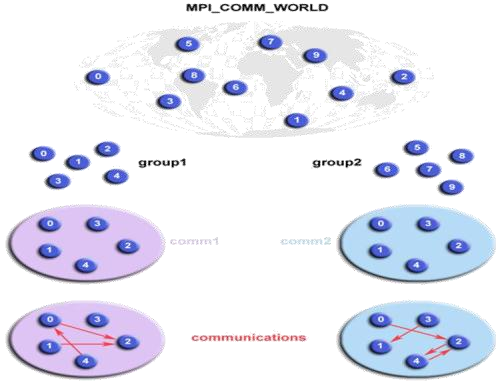
\includegraphics{MPI_04.png}
\newpage

\textbf{Level of Thread Support:} \\ 
MPI libraries vary in their level of thread support: \\
\begin{itemize}
	\item	MPI\_THREAD\_SINGLE - Level 0: Only one thread will execute.  
	\item	MPI\_THREAD\_FUNNELED - Level 1: The process may be multi-threaded, but only the main thread will make MPI calls - all MPI calls are funneled to the main  thread.  
	\item	MPI\_THREAD\_SERIALIZED - Level 2: The process may be multi-threaded, and multiple threads may make MPI calls, but only one at a time. That is, calls are 
	not made concurrently from two distinct threads as all MPI calls are serialized.  
	\item	MPI\_THREAD\_MULTIPLE - Level 3: Multiple threads may call MPI with no restrictions.
\end{itemize}	 
  
\textbf{Pros of MPI:} 
\begin{itemize}
	\item  runs on either shared or distributed memory architectures 
	\item  can be used on a wider range of problems than OpenMP 
	\item  each process has its own local variables 
	\item distributed memory computers are less expensive than large shared memory computers 
\end{itemize} 
 
\textbf{Cons of MPI:}  
\begin{itemize}
	\item requires more programming changes to go from serial to parallel version O can be harder to debug 
	\item  performance is limited by the communcation network between the nodes 
	
\end{itemize}

\newpage

\section{MPI Scatter, Gather:} 

MPI\_Gather( void* send\_data, int send\_count,  MPI\_Datatype send\_datatype, void* recv\_data, int recv\_count, MPI\_Datatype recv\_datatype,  	int root, MPI\_Comm communicator) \\ \\
MPI\_Bcast( void* data,  int count,  MPI\_Datatype datatype,  int root, MPI\_Comm communicator)

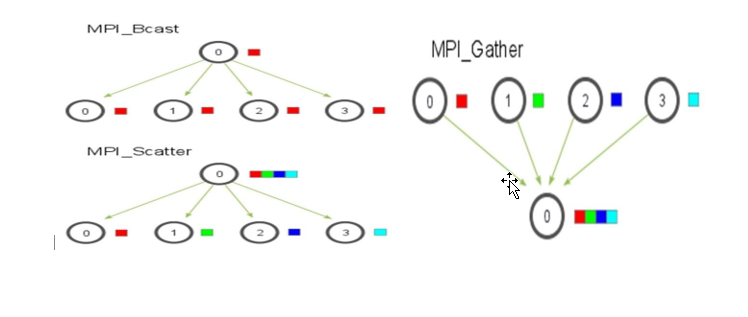
\includegraphics[scale=0.75]{MPI_06}

\section{Testing}
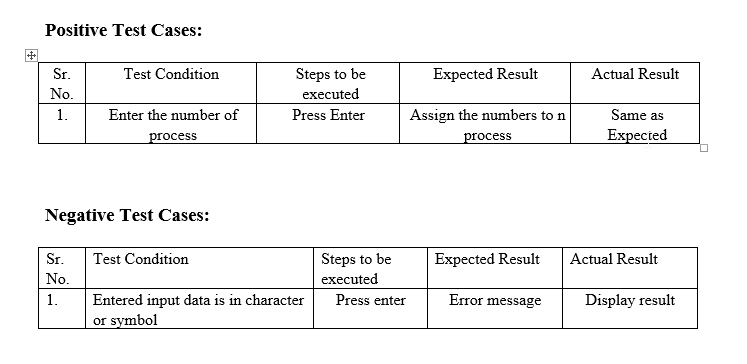
\includegraphics[scale=0.75]{MPI_07}

\section{Algorithm}
\begin{enumerate}
	\item Start
    \item Initialize array $x$
    \item Copy $x[0]$ to an integer $f$
    \item Send i-th element to i-th processor using $MPI\_Send()$
    \item Every worker receives it's $f$ from the manager
    \item Every worker performs square operation
    \item The workers send the result back to manager using $MPI\_Send()$
    \item Manager receives the result using $MPI\_Receive()$
    \item The time required is calculated by using $MPI\_Wtime()$
    \item Stop
\end{enumerate}

\section{Conclusion}
	\paragraph{} Thus, we have implemented a MPI Program for calculating a quantity called coverage from data files. 
\vspace{20px}
\begin{center}
	\begin{tabular}
		{|c|c|c|c|}\hline
		{\bf Roll No.}		&{\bf Name of Student}		&{\bf Date of Performance}  				&{\bf Date of Submission}  \\ \hline
		{302}	&	{Abhinav Bakshi}& {30/12/16}		& { 6/1/16}\\ \hline
	\end{tabular}\\ 
\end{center}

\section{Plagarism Report}
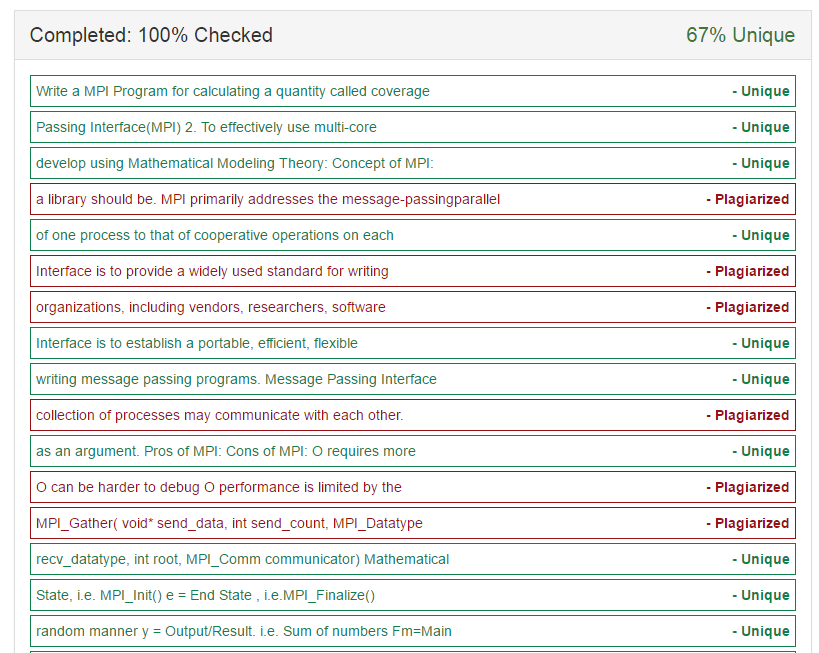
\includegraphics[scale=0.75]{mpi_plagarism}
\end{document}
 

 
